The advent of ChatGPT has significantly impacted both academia and industry due to its interactive capabilities and widespread application, establishing itself as a leading artificial intelligence tool \cite{DBLP:journals/corr/abs-2305-18486, DBLP:journals/corr/abs-2306-04504, DBLP:journals/corr/abs-2402-11203}. At the core of ChatGPT is the large language model (LLM) GPT-4, as detailed by \cite{achiam2023gpt}, which has seen numerous enhancements to its predecessors, showcasing exceptional abilities in a variety of Natural Language Processing (NLP) tasks \cite{DBLP:conf/ai/LaskarHH20}. Despite these advancements, the adoption of LLMs has highlighted several critical issues primarily due to their reliance on extensive datasets. This reliance restricts their ability to incorporate new information post-training, leading to three primary challenges. First, the focus on broad and general data to maximize accessibility and applicability results in subpar performance in specialized areas. Second, the rapid creation of online data, combined with the significant resources required for data annotation and model training, hinders LLMs' ability to stay updated. Third, LLMs are susceptible to generating convincing yet inaccurate responses, known as ``hallucinations'', which can mislead users.

\begin{figure}[t]
	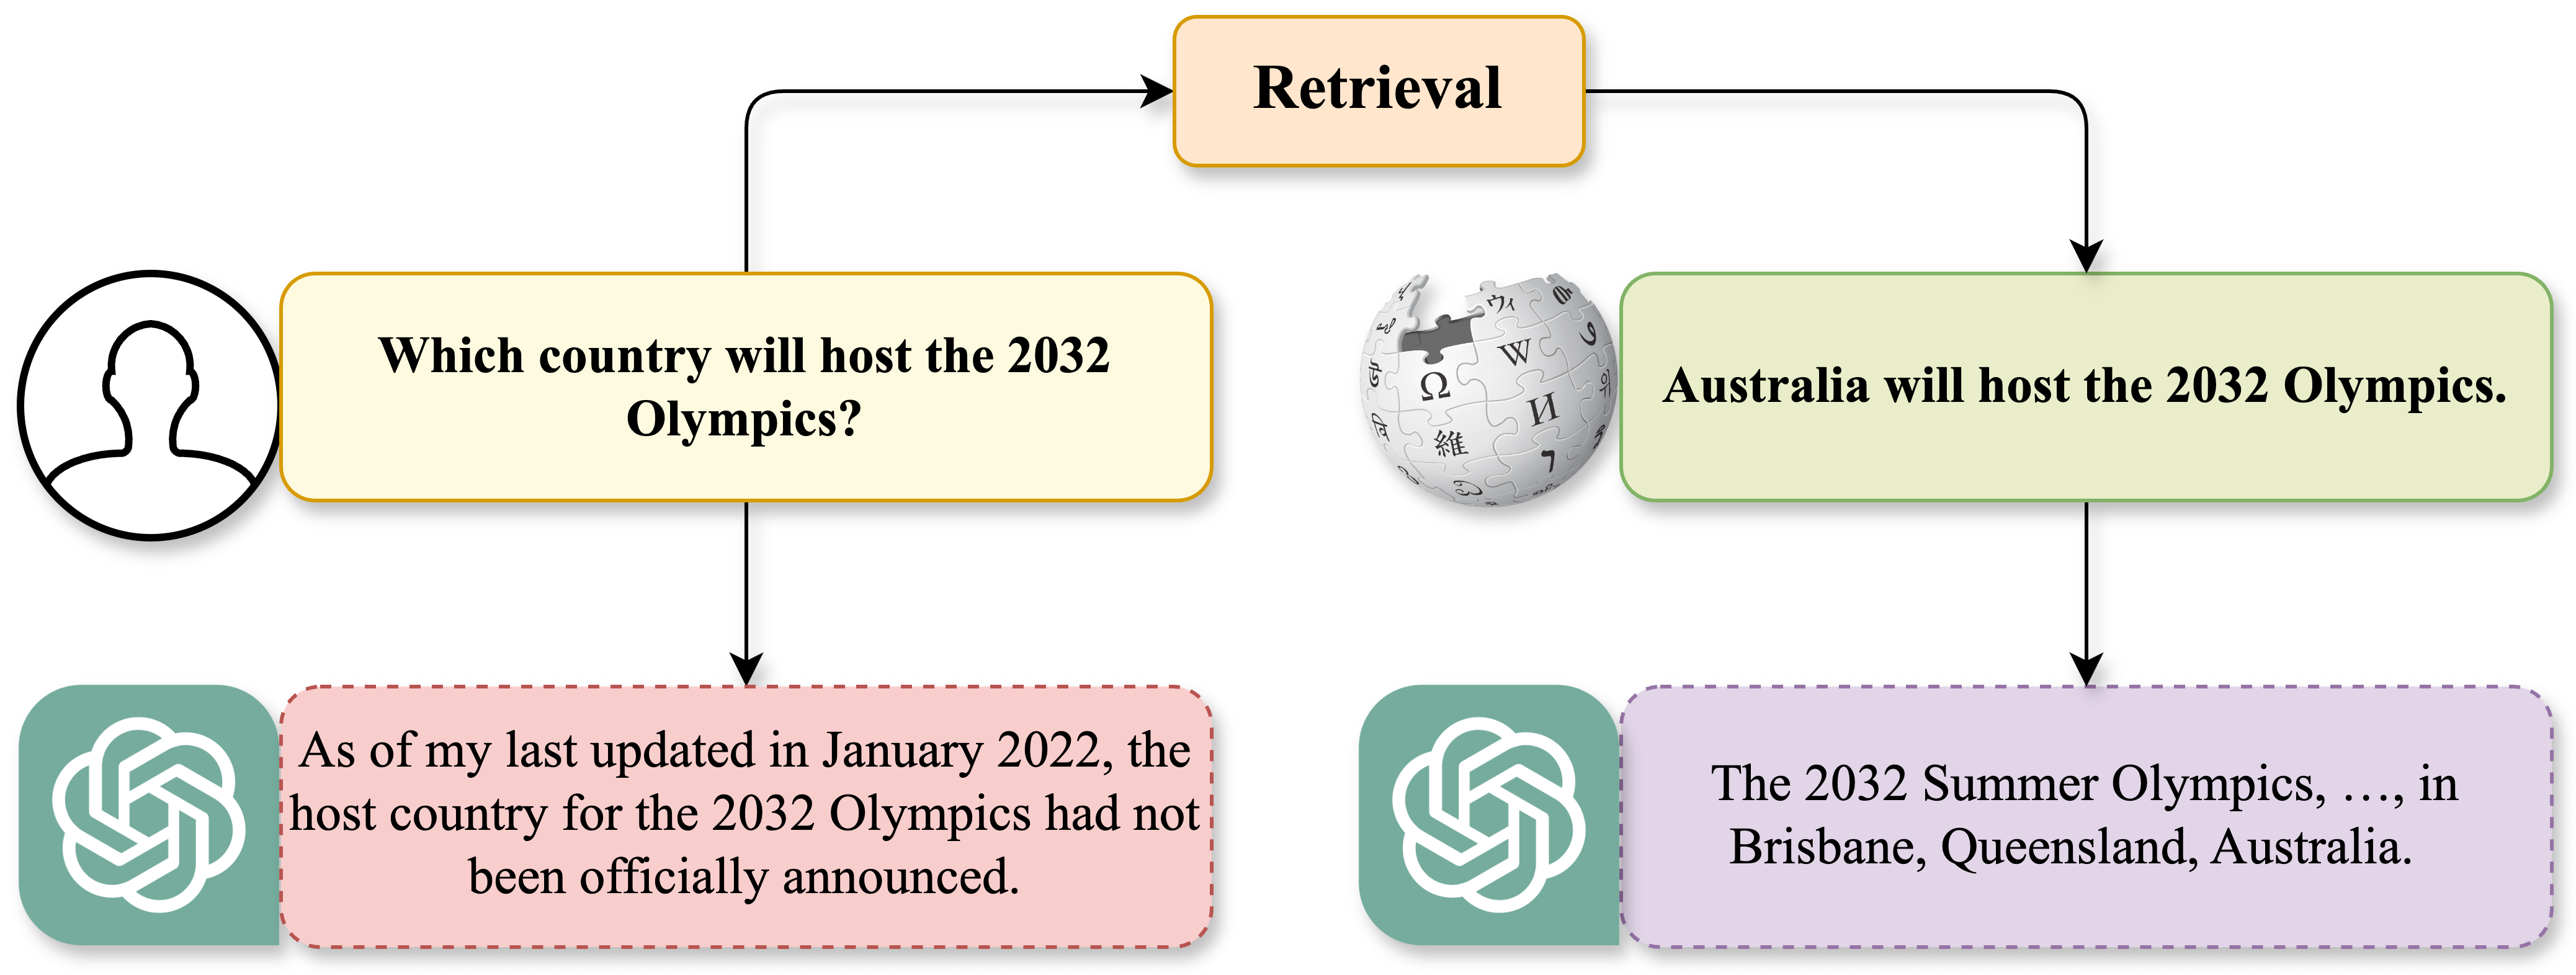
\includegraphics[width=0.6\textwidth]{Figures/RAG_example.png}
	\caption{An example of RAG benefits ChatGPT resolves questions that cannot be answered beyond the scope of the training data and generates correct results.}
	\label{fig:ragexample}
\end{figure}



Addressing these challenges is crucial for LLMs to be effectively utilized across various domains. A promising solution is the integration of Retrieval-Augmented Generation (RAG) technology, which supplements models by fetching external data in response to queries, thus ensuring more accurate and current outputs. Figure~\ref{fig:ragexample} illustrates how RAG can enable ChatGPT to provide precise answers beyond its initial training data.

Since its introduction by Lewis et al. \cite{lewis2020retrievalaugmented} in 2020, RAG has seen rapid development, especially with the rise of models like ChatGPT. Despite these advancements, there remains a noticeable gap in the literature regarding a comprehensive analysis of the mechanisms underlying RAG and the progress achieved by subsequent studies. Moreover, the field suffers from fragmented research focuses and inconsistent terminology for similar methods, leading to confusion. This survey seeks to bridge this gap by offering a structured overview of RAG, categorizing various approaches, and providing an in-depth understanding of the current research landscape, with a focus on textual applications given their prominence in recent research.

To provide clarity and structure, this paper is organized as follows: Section 2 outlines the overall RAG workflow, dividing the methodologies into pre-retrieval, retrieval, post-retrieval, and generation phases. Sections 3 through 6 explore the core techniques within each phase. Section 7 focuses on the evaluation methodologies for RAG. Section 8 summarizes the reviewed studies, detailing the retrievers and generators used, while Section 9 discusses challenges and future research directions, extending beyond text-based studies to include multimodal data applications. The paper concludes with Section 10.

Other related surveys provide valuable insights into the evolving RAG landscape from different angles. Gao et al. \cite{gao2023retrievalaugmented} identified three key stages in RAG development: pre-training enhancement, inference, and fine-tuning. Zhao et al. \cite{zhao2024retrievalaugmented} focused on the diverse applications of RAG, including text, code, image, and video generation, emphasizing augmented intelligence in generative tasks. Meanwhile, Hu et al. \cite{hu2024rau} explored Retrieval-Augmented Language Models (RALMs), examining how interactions between retrievers, language models, and augmentations influence model architectures and applications.

In this paper, we aim to offer a comprehensive and unified framework for understanding RAG from an information retrieval (IR) perspective, identifying key challenges and areas for improvement. We delve into the core technologies that drive RAG, assessing their effectiveness in addressing retrieval and generation tasks. Additionally, this survey introduces the evaluation methods employed in RAG research, highlights current limitations, and proposes promising avenues for future exploration.

